% Options for packages loaded elsewhere
\PassOptionsToPackage{unicode}{hyperref}
\PassOptionsToPackage{hyphens}{url}
\PassOptionsToPackage{dvipsnames,svgnames,x11names}{xcolor}
%
\documentclass[
  12pt,
]{article}
\usepackage{amsmath,amssymb}
\usepackage{lmodern}
\usepackage{iftex}
\ifPDFTeX
  \usepackage[T1]{fontenc}
  \usepackage[utf8]{inputenc}
  \usepackage{textcomp} % provide euro and other symbols
\else % if luatex or xetex
  \usepackage{unicode-math}
  \defaultfontfeatures{Scale=MatchLowercase}
  \defaultfontfeatures[\rmfamily]{Ligatures=TeX,Scale=1}
\fi
% Use upquote if available, for straight quotes in verbatim environments
\IfFileExists{upquote.sty}{\usepackage{upquote}}{}
\IfFileExists{microtype.sty}{% use microtype if available
  \usepackage[]{microtype}
  \UseMicrotypeSet[protrusion]{basicmath} % disable protrusion for tt fonts
}{}
\makeatletter
\@ifundefined{KOMAClassName}{% if non-KOMA class
  \IfFileExists{parskip.sty}{%
    \usepackage{parskip}
  }{% else
    \setlength{\parindent}{0pt}
    \setlength{\parskip}{6pt plus 2pt minus 1pt}}
}{% if KOMA class
  \KOMAoptions{parskip=half}}
\makeatother
\usepackage{xcolor}
\usepackage[margin=1in]{geometry}
\usepackage{longtable,booktabs,array}
\usepackage{calc} % for calculating minipage widths
% Correct order of tables after \paragraph or \subparagraph
\usepackage{etoolbox}
\makeatletter
\patchcmd\longtable{\par}{\if@noskipsec\mbox{}\fi\par}{}{}
\makeatother
% Allow footnotes in longtable head/foot
\IfFileExists{footnotehyper.sty}{\usepackage{footnotehyper}}{\usepackage{footnote}}
\makesavenoteenv{longtable}
\usepackage{graphicx}
\makeatletter
\def\maxwidth{\ifdim\Gin@nat@width>\linewidth\linewidth\else\Gin@nat@width\fi}
\def\maxheight{\ifdim\Gin@nat@height>\textheight\textheight\else\Gin@nat@height\fi}
\makeatother
% Scale images if necessary, so that they will not overflow the page
% margins by default, and it is still possible to overwrite the defaults
% using explicit options in \includegraphics[width, height, ...]{}
\setkeys{Gin}{width=\maxwidth,height=\maxheight,keepaspectratio}
% Set default figure placement to htbp
\makeatletter
\def\fps@figure{htbp}
\makeatother
\setlength{\emergencystretch}{3em} % prevent overfull lines
\providecommand{\tightlist}{%
  \setlength{\itemsep}{0pt}\setlength{\parskip}{0pt}}
\setcounter{secnumdepth}{5}
\newlength{\cslhangindent}
\setlength{\cslhangindent}{1.5em}
\newlength{\csllabelwidth}
\setlength{\csllabelwidth}{3em}
\newlength{\cslentryspacingunit} % times entry-spacing
\setlength{\cslentryspacingunit}{\parskip}
\newenvironment{CSLReferences}[2] % #1 hanging-ident, #2 entry spacing
 {% don't indent paragraphs
  \setlength{\parindent}{0pt}
  % turn on hanging indent if param 1 is 1
  \ifodd #1
  \let\oldpar\par
  \def\par{\hangindent=\cslhangindent\oldpar}
  \fi
  % set entry spacing
  \setlength{\parskip}{#2\cslentryspacingunit}
 }%
 {}
\usepackage{calc}
\newcommand{\CSLBlock}[1]{#1\hfill\break}
\newcommand{\CSLLeftMargin}[1]{\parbox[t]{\csllabelwidth}{#1}}
\newcommand{\CSLRightInline}[1]{\parbox[t]{\linewidth - \csllabelwidth}{#1}\break}
\newcommand{\CSLIndent}[1]{\hspace{\cslhangindent}#1}
\usepackage{polyglossia}
\setmainlanguage{english}
\usepackage{booktabs}
\usepackage{caption}
\captionsetup[table]{skip=10pt}
\ifLuaTeX
  \usepackage{selnolig}  % disable illegal ligatures
\fi
\IfFileExists{bookmark.sty}{\usepackage{bookmark}}{\usepackage{hyperref}}
\IfFileExists{xurl.sty}{\usepackage{xurl}}{} % add URL line breaks if available
\urlstyle{same} % disable monospaced font for URLs
\hypersetup{
  pdftitle={Potato resources and use in Russia},
  pdfauthor={Kerimov Gasym},
  colorlinks=true,
  linkcolor={Maroon},
  filecolor={Maroon},
  citecolor={Blue},
  urlcolor={blue},
  pdfcreator={LaTeX via pandoc}}

\title{Potato resources and use in Russia}
\author{Kerimov Gasym}
\date{}

\begin{document}
\maketitle

\textbf{\emph{Research question }}

How have changes in potato resource availability and use impacted the food security and economic development of Russia?

\textbf{Introduction}

Potatoes are a staple food in Russian cuisine and have been a crucial resource for the country for centuries. Over the years, the availability and use of potatoes have undergone significant changes in Russia due to various factors such as economic and political transitions, technological advancements, and climate change. Understanding the historical and current trends in potato resources and use in Russia can shed light on their impact on the country's food security and economic development. The dataset includes information on details, such as:

\begin{itemize}
\item
  \textbf{Stocks at the beginning of the year}
\item
  \textbf{Production}
\item
  \textbf{Imports, including imports}
\item
  \textbf{Total Resources}
\item
  \textbf{Productive consumption}
\item
  \textbf{Losses}
\item
  \textbf{Export,including export}
\item
  \textbf{Personal consumption }
\item
  \textbf{Stocks at the end of the year }
\end{itemize}

This study aims to examine the historical and current trends in potato resources and use in Russia and analyze their impact on the country's food security and economic development. By using both primary and secondary sources of data, including official statistics, scholarly articles, and expert interviews, this study will provide an in-depth analysis of the various factors that have influenced the potato industry in Russia over time. The findings of this research will contribute to a better understanding of the importance of potato resources and use in Russia and can inform policies aimed at improving food security and economic development in the country.

\begin{figure}
\centering
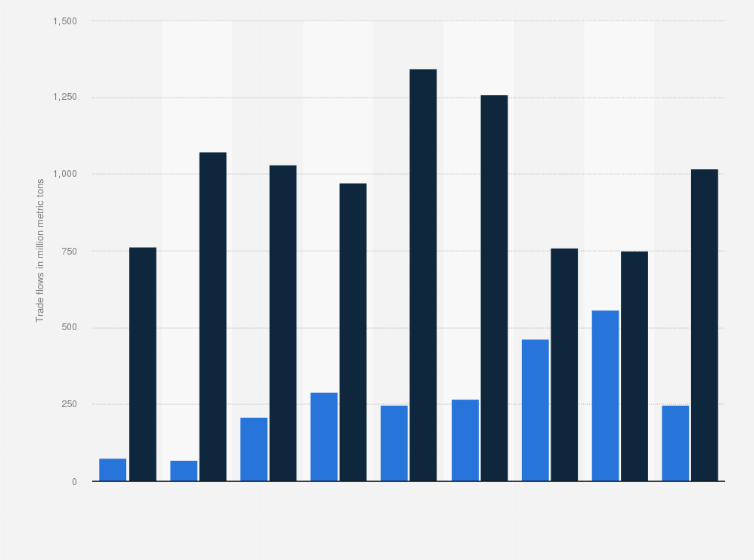
\includegraphics{static/img/1270064-blank-754}
\caption{alt text}
\end{figure}

Potato is an important crop in the world and in our country. Gross production is more than 370 million tons. More than half of the world production is in developing countries for the
nutrition of the population. In Russia, it is also a fundamental element of the food security of the country, since the basis of the population's nutrition is bread and potatoes. Its economic value is also increasing due to the use of potato starch for various purposes - from confectionery production to
oil drilling.
According to FAO, China, India and Russia are the main producers of gross potato. However, gross production is not an indicator of industry development. The main indicator is crop productivity. In terms of productivity, Russia is in one of the last places. According to FAOSTAT, the average
world productivity in 2016 was 19.6 t·ha-1, in Russia -- 14.6. The yield growth of this crop is observed in all countries and continents; the world rating is headed by the USA and New Zealand, where the average yield was 49.0 t·ha-1

As stated in the World Bank report, the growth of agricultural production is the engine of the development of related industries, and in general the economies of low-income countries (World Bank, 2007), which is confirmed by numerous research.

In such conditions, the global market promotes the development of regional agricultural enterprises. The processes of economic integration and trade liberalization have a significant impact on market volumes and food security (Demichev, 2019). The latter problem is urgent for potato markets in many countries of the world.

Availability of the agri-food market at the national and regional levels creates prerequisites for the development of export-oriented industries, although it is accompanied by objective difficulties in promoting products to final consumers.

The problem of realizing the growth potential of agricultural producers is solved differently in various studies. Some researchers consider the rational placement of production as the basis for production development, taking into account natural factors, such as seasonality.

\hypertarget{literature-review}{%
\subsection{Literature Review}\label{literature-review}}

New citation for my article Sokolov et al. (\protect\hyperlink{ref-sokolov2020complex}{2020}) or I can type (\protect\hyperlink{ref-sokolov2020complex}{Sokolov et al., 2020})

New citation for my article Animitsa et al. (\protect\hyperlink{ref-animitsa2014evolution}{2014}) or I can type (\protect\hyperlink{ref-animitsa2014evolution}{Animitsa et al., 2014})

New citation for my article Ivashova et al. (\protect\hyperlink{ref-ivashova2020justification}{2020}) or I can type (\protect\hyperlink{ref-ivashova2020justification}{Ivashova et al., 2020})

New citation for my article Demichev (\protect\hyperlink{ref-demichev2019sustainable}{2019}) or I can type (\protect\hyperlink{ref-demichev2019sustainable}{Demichev, 2019})

\newpage

\hypertarget{references}{%
\section{References}\label{references}}

\hypertarget{refs}{}
\begin{CSLReferences}{1}{0}
\leavevmode\vadjust pre{\hypertarget{ref-animitsa2014evolution}{}}%
Animitsa, Y. G., Animitsa, P. Y., \& Denisova, O. Y. (2014). Evolution of knowledge about distribution of productive forces. \emph{Economy of Region/Ekonomika Regiona}, \emph{38}(2).

\leavevmode\vadjust pre{\hypertarget{ref-demichev2019sustainable}{}}%
Demichev, V. (2019). Sustainable development of agriculture based on inclusiveness. \emph{Economics of Agriculture in Russia}, \emph{6}, 32.

\leavevmode\vadjust pre{\hypertarget{ref-ivashova2020justification}{}}%
Ivashova, O., Gasparyan, I., Levshin, A., \& Dyikanova, M. (2020). Justification of possibility of cultivating in moscow region two-crop culture of early potatoes. \emph{Engineering for Rural Development}, \emph{19}, 399--405.

\leavevmode\vadjust pre{\hypertarget{ref-sokolov2020complex}{}}%
Sokolov, N., Belous, N., Torikov, B., \& Babiak, M. (2020). Integrated development of bioresources in rural areas: Theory, practice, problems. \emph{Bulletin of the Bryansk State Agricultural Academy}, \emph{2 (78)}, 56--65.

\end{CSLReferences}

\end{document}
